% !TeX program = lualatex
% ================================================================
% Polish Tier 3 Vocabulary Version of ChineseMultiplicationMethod
%
% Generated by the server using the following settings:
%
%   language            Polish (pol)
%   text direction      left to right
%   font                Noto Serif
%   fallback font       Noto Serif
%   built from          latex/worksheets/arithmetic/chineseMultiplicationMethod.tex
%   vocabulary key      latex/worksheets/arithmetic/chineseMultiplicationMethod/L2/pol/chineseMultiplicationMethod_polishKey.tex
%   tier 3 vocabulary   green   RGB 0 128 0
%   English text        black   RGB 0 0 0
%   Polish text         purple  RGB 112 48 160
%   layout macros       version 3
%
% Please don't edit any information in this comment block - the server
% compares it against the current settings and rebuilds this file when
% they differ, so changes here would be overwritten. However, feel free
% to make updates to the LaTeX below if you want to edit it.
% ================================================================

\documentclass[12pt,a4paper]{article}
% ================================================================
% Copied from the English sheet this was translated from, so that
% anything it sets up for itself still works here
% ================================================================
\usepackage[a4paper,top=12mm,bottom=14mm,left=15mm,right=15mm]{geometry}
\usepackage[T1]{fontenc}
\usepackage{amsmath}
\usepackage{amssymb}
\usepackage{enumitem}
\usepackage{multicol}
\usepackage{tikz}
\usepackage[most]{tcolorbox}
\usetikzlibrary{arrows.meta}

% ================================================================
% The Chinese multiplication method.
%
% A Key Stage 3 arithmetic sheet, designed to be worked through
% alone: the method is introduced by a worked example, then
% practised in three stages of decreasing support -- a grid that is
% already filled in, so that only the diagonal addition is left; a
% grid that is drawn but empty; and finally no grid at all. The
% decimal point runs through the whole sheet, first with both
% numbers written as decimals and then with one of them whole.
% Answers are on the last page so that pupils can check each part
% before going on.
%
% The sheet is written on, so every question is followed by a
% working area. The \newpage commands in the body are placed so
% that no question is split across the fold.
% ================================================================

\pagestyle{empty}
\linespread{1.15}\selectfont
\setlength{\parskip}{5pt}
\setlist[enumerate,1]{label=\textbf{Q\arabic*.}, leftmargin=*, itemsep=10pt, topsep=6pt, parsep=4pt}
\setlist[enumerate,2]{label=(\alph*), leftmargin=*, itemsep=8pt, topsep=5pt, parsep=3pt}
\setlength{\multicolsep}{4pt}
\setlength{\parindent}{0pt}

\newcommand{\ansline}[1][2.2cm]{\underline{\hspace{#1}}}

% A worked example: the method shown in full before it is practised.
\newtcolorbox{wex}[1]{colback=blue!4,colframe=blue!45!black,boxrule=0.6pt,
  left=6pt,right=6pt,top=4pt,bottom=5pt,
  title={\bfseries\small Worked example: #1},fonttitle=\small,
  toptitle=1pt,bottomtitle=1pt}

% The idea a section is built on, stated once and boxed.
\newtcolorbox{keyidea}{colback=orange!7,colframe=orange!60!black,boxrule=0.6pt,
  left=6pt,right=6pt,top=4pt,bottom=4pt}

% The section headings, kept tight so the parts do not eat the page.
\newcommand{\heading}[1]{%
  \vspace{2pt}
  {\color{blue!45!black}\rule{\linewidth}{1pt}}\\[1pt]
  {\large\bfseries #1}\\[-6pt]
  {\color{blue!45!black}\rule{\linewidth}{0.4pt}}
  \vspace{2pt}}
\newcommand{\parttitle}[2]{\heading{Part #1: #2}}

% ----------------------------------------------------------------
% The Chinese multiplication grid.
%
% \lsetup{<columns>}{<rows>} records the size of the grid that the
% macros below draw into; every coordinate is worked out from it, so
% a grid is resized by changing that one line. Columns are numbered
% from the left and rows from the top, so cell (i,j) holds the
% product of digit i of the number along the top and digit j of the
% number down the side. One cell is one unit square, and the
% diagonals run from the bottom left corner of a cell to its top
% right corner, which puts the tens digit of a product above the
% diagonal and the units digit below it.
%
% A grid needs at least two columns and two rows: \foreach counts
% downwards through {1,...,0}, so a single column would draw its
% internal lines in the wrong place.
\newcommand{\lsetup}[2]{%
  \edef\lC{\the\numexpr#1\relax}\edef\lR{\the\numexpr#2\relax}%
  \edef\lCm{\the\numexpr#1-1\relax}\edef\lRm{\the\numexpr#2-1\relax}}

\newcommand{\lgrid}{%
  \draw[thick] (0,0) rectangle (\lC,\lR);
  \foreach \i in {1,...,\lCm}{\draw (\i,0) -- (\i,\lR);}
  \foreach \j in {1,...,\lRm}{\draw (0,\j) -- (\lC,\j);}
  \foreach \i in {1,...,\lC}{\foreach \j in {1,...,\lR}{%
    \draw[gray!75] ({\i-1},{\j-1}) -- (\i,\j);}}}

% The two numbers being multiplied: \ltop along the columns,
% \lside down the rows.
\newcommand{\ltop}[2]{\node[font=\small] at ({#1-0.5},{\lR+0.34}) {#2};}
\newcommand{\lside}[2]{\node[font=\small] at ({\lC+0.34},{\lR-#1+0.5}) {#2};}

% One cell: #3 above the diagonal, #4 below it.
\newcommand{\lcell}[4]{%
  \node[font=\small] at ({#1-0.72},{\lR-#2+0.70}) {#3};
  \node[font=\small] at ({#1-0.28},{\lR-#2+0.30}) {#4};}

% The digits of the answer, read down the left side and then along
% the bottom, and the writing lines they are written on.
\newcommand{\lleft}[2]{\node[font=\small] at (-0.44,{\lR-#1+0.5}) {#2};}
\newcommand{\lbot}[2]{\node[font=\small] at ({#1-0.5},-0.42) {#2};}
\newcommand{\lanslines}{%
  \foreach \j in {1,...,\lR}{\draw[gray!60] (-0.74,{\lR-\j+0.28}) -- (-0.14,{\lR-\j+0.28});}
  \foreach \i in {1,...,\lC}{\draw[gray!60] ({\i-0.8},-0.6) -- ({\i-0.2},-0.6);}}

% The decimal points of the two numbers, marked on the edge of the
% grid between the two digits each one separates. \ltopdot{k} sits
% after the kth column and \lsidedot{k} after the kth row, so a
% whole number carries its mark on the corner of the grid.
\newcommand{\ltopdot}[1]{\fill (#1,{\lR+0.2}) circle (1.8pt);}
\newcommand{\lsidedot}[1]{\fill ({\lC+0.34},{\lR-#1}) circle (1.8pt);}

% Where the decimal point of the answer goes. The line down from the
% top mark and the line in from the side mark meet at a corner of a
% cell; the diagonal from that corner leaves the grid at (\lex,\ley),
% and the point is written just outside it at (\ldx,\ldy).
\newcommand{\lmeet}[2]{%
  \pgfmathsetmacro{\lmx}{#1}%
  \pgfmathsetmacro{\lmy}{\lR-#2}%
  \pgfmathsetmacro{\lts}{min(\lmx,\lmy)}%
  \pgfmathsetmacro{\lex}{\lmx-\lts}%
  \pgfmathsetmacro{\ley}{\lmy-\lts}%
  \pgfmathsetmacro{\ldx}{\lex<0.5 ? -0.44 : \lex}%
  \pgfmathsetmacro{\ldy}{\ley<0.5 ? -0.42 : \ley}}
\newcommand{\lansdot}[2]{\lmeet{#1}{#2}%
  \fill[red!75!black] ({\ldx},{\ldy}) circle (2.1pt);}
\newcommand{\ltrace}[2]{\lmeet{#1}{#2}%
  \draw[red!75!black,dashed,-{Stealth[length=2mm]}] ({\lmx},{\lR+0.1}) -- ({\lmx},{\lmy});
  \draw[red!75!black,dashed,-{Stealth[length=2mm]}] ({\lC+0.12},{\lmy}) -- ({\lmx},{\lmy});
  \ifdim\lts pt>0.1pt
    \draw[red!75!black,dashed,thick,-{Stealth[length=2mm]}] ({\lmx},{\lmy}) -- ({\lex},{\ley});
  \fi
  \fill[red!75!black] ({\ldx},{\ldy}) circle (2.1pt);}

% The order the answer is read in.
\newcommand{\lreadarrow}{%
  \draw[gray,rounded corners=5pt,-{Stealth[length=2.2mm]}]
    (-1.0,{\lR-0.2}) -- (-1.0,-0.95) -- ({\lC+0.05},-0.95);}

% Characters this language's font has not got are borrowed from another,
% rather than being silently dropped - see docs/translated-sheet-latex.md
\directlua{%
  if luaotfload and luaotfload.add_fallback then
    luaotfload.add_fallback("eallatinfallback",
      { "Noto Serif:mode=harf;" })
  else
    tex.error("this luaotfload is too old to register a fallback font")
  end
}
\usepackage[english]{babel}
\babelprovide[import]{polish}
\babelfont[polish]{rm}[Renderer=Harfbuzz, BoldFont={Noto Serif}, ItalicFont={Noto Serif}, BoldItalicFont={Noto Serif}, RawFeature={fallback=eallatinfallback}]{Noto Serif}
\babelfont[polish]{sf}[Renderer=Harfbuzz, BoldFont={Noto Serif}, ItalicFont={Noto Serif}, BoldItalicFont={Noto Serif}, RawFeature={fallback=eallatinfallback}]{Noto Serif}
\newcommand{\ealtext}[1]{\foreignlanguage{polish}{#1}}
\newcommand{\ealtextblock}[1]{{\raggedright\foreignlanguage{polish}{#1}\par}}
% ================================================================
% EAL layout helpers
% ================================================================
\usepackage{xcolor}

\definecolor{ealkeycolour}{RGB}{0,128,0}
\definecolor{ealenglish}{RGB}{0,0,0}
\definecolor{ealtwocolour}{RGB}{112,48,160}

\newsavebox{\ealboxen}
\newsavebox{\ealboxtr}
\newlength{\ealglosswd}
\newlength{\ealglossraise}
\setlength{\ealglossraise}{1.15em}

% a tier 3 word, in English and in translation alike
\newcommand{\ealkey}[1]{\textcolor{ealkeycolour}{#1}}
\newcommand{\ealkeytr}[1]{\textcolor{ealkeycolour}{\ealtext{#1}}}

% One translated word above one English word. Built from kernel
% primitives, never a tabular, which would break wherever the sheet
% loads array, booktabs or tabularx. The box is as wide as the wider of
% the two, so a long translation pushes its neighbours aside instead of
% overlapping them, and it claims its full height so a table row or a
% TikZ node makes room for it.
\newcommand{\ealgloss}[2]{%
  \sbox{\ealboxen}{\ealkey{#1}}%
  \sbox{\ealboxtr}{\small\textcolor{ealtwocolour}{\ealtext{#2}}}%
  \setlength{\ealglosswd}{\wd\ealboxen}%
  \ifdim\wd\ealboxtr>\ealglosswd\setlength{\ealglosswd}{\wd\ealboxtr}\fi
  \leavevmode
  \makebox[\ealglosswd][c]{%
    \makebox[0pt][c]{\usebox{\ealboxen}}%
    \makebox[0pt][c]{\raisebox{\ealglossraise}{\usebox{\ealboxtr}}}%
  }%
}

% opens up line spacing around a block of glosses, so the raised
% translations sit clear of the line above
\newenvironment{ealglossed}{\par\linespread{2.1}\selectfont\ignorespaces}{\par}

% a whole translated sentence above its English counterpart. block level,
% so it does not belong inside a tabular cell
\newcommand{\ealpara}[2]{%
  \par\addvspace{0.5\baselineskip}%
  {\color{ealtwocolour}\ealtextblock{#1}}%
  \penalty200
  {\color{ealenglish}#2\par}%
  \addvspace{0.5\baselineskip}%
}

\begin{document}

\begin{ealglossed}
\begin{center}
  {\Large\bfseries The \ealgloss{Lattice}{krata} \ealgloss{Multiplication}{mnożyć} Method}\\[6pt]
\end{center}
\end{ealglossed}

\begin{ealglossed}
The \ealgloss{lattice}{krata} method, sometimes called the Chinese method, is a \ealgloss{multiplication}{mnożyć} method that uses a \ealgloss{grid}{siatka} to organise the calculation.
\end{ealglossed}

\begin{ealglossed}
\parttitle{1}{\ealgloss{Multiplying}{mnożyć} two \ealgloss{whole numbers}{liczby całkowite nieujemne}}
\end{ealglossed}

\begin{ealglossed}
We draw a \ealgloss{grid}{siatka} (sometimes called a \ealgloss{lattice}{krata}), the number of \ealgloss{rows}{wiersze} and \ealgloss{columns}{kolumny} should match the number of \ealgloss{digits}{cyfry} in the two numbers we are \ealgloss{multiplying}{mnożyć}.
\end{ealglossed}

\begin{ealglossed}
For example $47 \times 36$ is \ealgloss{multiplying}{mnożyć} a 2 \ealgloss{digit}{cyfra} number by a 2 \ealgloss{digit}{cyfra} number, so our \ealgloss{grid}{siatka} would have 2 \ealgloss{columns}{kolumny} and 2 \ealgloss{rows}{wiersze}.
\end{ealglossed}

\begin{ealglossed}
Each \ealgloss{cell}{komórka} of the \ealgloss{grid}{siatka} is split diagonally, and we write the \ealgloss{product}{iloczyn} of the \ealgloss{digits}{cyfry} in the \ealgloss{cell}{komórka}, with the \ealgloss{tens digit}{cyfra dziesiątek} above the \ealgloss{diagonal}{przekątna} and the \ealgloss{units digit}{cyfra jedności} below it.
\end{ealglossed}

\begin{ealglossed}
Finally we add along the \ealgloss{diagonals}{przekątne}, starting from the bottom right corner. If a \ealgloss{diagonal}{przekątna} adds up to more than ten, we \ealgloss{carry}{przenosić} into the next \ealgloss{diagonal}{przekątna}.
\end{ealglossed}

\begin{wex}{$47\times36$}
\small
\begin{minipage}[t]{0.44\linewidth}
\centering
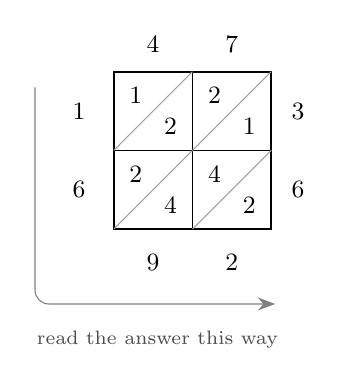
\begin{tikzpicture}[baseline=(current bounding box.north),scale=1.0]
  \lsetup{2}{2}
  \lgrid
  \ltop{1}{4} \ltop{2}{7}
  \lside{1}{3} \lside{2}{6}
  \lcell{1}{1}{1}{2} \lcell{2}{1}{2}{1}
  \lcell{1}{2}{2}{4} \lcell{2}{2}{4}{2}
  \lleft{1}{1} \lleft{2}{6}
  \lbot{1}{9} \lbot{2}{2}
  \lreadarrow
  \node[font=\scriptsize,gray!60!black,anchor=west] at (-1.1,-1.4)
    {read the answer this way};
\end{tikzpicture}
\end{minipage}%
\begin{minipage}[t]{0.56\linewidth}
\vspace{2pt}
$4\times3=12$, \; $7\times3=21$, \; $4\times6=24$, \; $7\times6=42$

\smallskip
\begin{ealglossed}
Adding the \ealgloss{diagonals}{przekątne}, starting from the bottom right corner:
\vspace{-2pt}
\begin{align*}
  \text{1st \ealgloss{diagonal}{przekątna}:}\quad & 2 && = 2\\[2pt]
  \text{2nd \ealgloss{diagonal}{przekątna}:}\quad & 4+4+1 && = 9\\[2pt]
  \text{3rd \ealgloss{diagonal}{przekątna}:}\quad & 2+2+2 && = 6\\[2pt]
  \text{4th \ealgloss{diagonal}{przekątna}:}\quad & 1 && = 1
\end{align*}
\end{ealglossed}
\vspace{-14pt}

So $47\times36=1692$.
\end{minipage}
\end{wex}

\begin{enumerate}

\item
\begin{ealglossed}
Both \ealgloss{grids}{siatki} below are already filled in. Add along the
\ealgloss{diagonals}{przekątne} and
write the answer. One \ealgloss{diagonal}{przekątna} in part (b) adds up to more than ten, so you
will need to \ealgloss{carry}{przenosić}.
\end{ealglossed}
\vspace{2pt}

\begin{minipage}[t]{0.5\linewidth}
\centering
(a) $52\times34$\\[4pt]
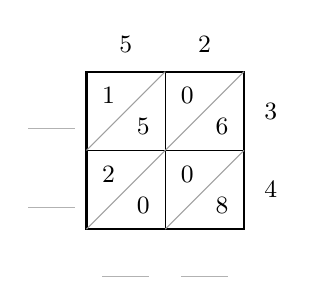
\begin{tikzpicture}[baseline=(current bounding box.north),scale=1.0]
  \lsetup{2}{2}
  \lgrid
  \ltop{1}{5} \ltop{2}{2}
  \lside{1}{3} \lside{2}{4}
  \lcell{1}{1}{1}{5} \lcell{2}{1}{0}{6}
  \lcell{1}{2}{2}{0} \lcell{2}{2}{0}{8}
  \lanslines
\end{tikzpicture}\\[8pt]
$52\times34=\ansline[2cm]$
\end{minipage}%
\begin{minipage}[t]{0.5\linewidth}
\centering
(b) $68\times47$\\[4pt]
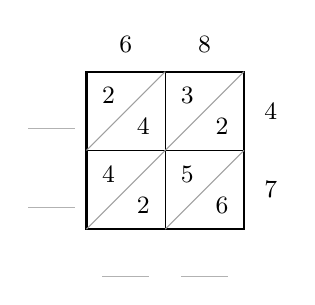
\begin{tikzpicture}[baseline=(current bounding box.north),scale=1.0]
  \lsetup{2}{2}
  \lgrid
  \ltop{1}{6} \ltop{2}{8}
  \lside{1}{4} \lside{2}{7}
  \lcell{1}{1}{2}{4} \lcell{2}{1}{3}{2}
  \lcell{1}{2}{4}{2} \lcell{2}{2}{5}{6}
  \lanslines
\end{tikzpicture}\\[8pt]
$68\times47=\ansline[2cm]$
\end{minipage}

\newpage

\item
\begin{ealglossed}
These \ealgloss{grids}{siatki} are drawn but empty. Fill in every \ealgloss{cell}{komórka}, then add along the
\ealgloss{diagonals}{przekątne}. Part (b) has a three-\ealgloss{digit}{cyfra} number, so its \ealgloss{grid}{siatka} has three \ealgloss{columns}{kolumny}.
\end{ealglossed}
\vspace{2pt}

\begin{minipage}[t]{0.42\linewidth}
\centering
(a) $34\times25$\\[4pt]
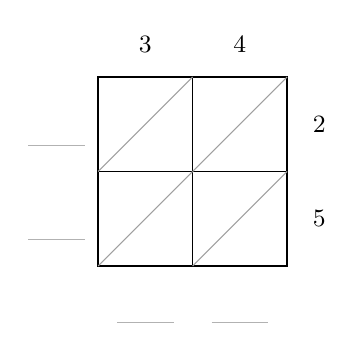
\begin{tikzpicture}[baseline=(current bounding box.north),scale=1.2]
  \lsetup{2}{2}
  \lgrid
  \ltop{1}{3} \ltop{2}{4}
  \lside{1}{2} \lside{2}{5}
  \lanslines
\end{tikzpicture}\\[8pt]
$34\times25=\ansline[2cm]$
\end{minipage}%
\begin{minipage}[t]{0.58\linewidth}
\centering
(b) $243\times17$\\[4pt]
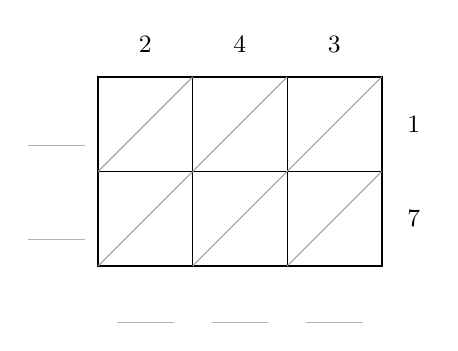
\begin{tikzpicture}[baseline=(current bounding box.north),scale=1.2]
  \lsetup{3}{2}
  \lgrid
  \ltop{1}{2} \ltop{2}{4} \ltop{3}{3}
  \lside{1}{1} \lside{2}{7}
  \lanslines
\end{tikzpicture}\\[8pt]
$243\times17=\ansline[2cm]$
\end{minipage}

\end{enumerate}

\begin{ealglossed}
\parttitle{2}{Where the \ealgloss{decimal point}{przecinek dziesiętny} goes}
\end{ealglossed}

\begin{ealglossed}
The \ealgloss{lattice}{krata} method can also be used to \ealgloss{multiply}{mnożyć} \ealgloss{decimal numbers}{liczby dziesiętne}. The \ealgloss{decimal point}{przecinek dziesiętny} in the answer is located on the \ealgloss{diagonal}{przekątna} where the two \ealgloss{decimal points}{przecinki dziesiętne} in the numbers being \ealgloss{multiplied}{mnożyć} meet, as seen below.
\end{ealglossed}

\begin{wex}{$2.6\times3.4$}
\small
\begin{minipage}[t]{0.40\linewidth}
\centering
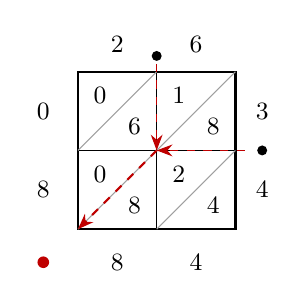
\begin{tikzpicture}[baseline=(current bounding box.north),scale=1.0]
  \lsetup{2}{2}
  \lgrid
  \ltop{1}{2} \ltop{2}{6} \ltopdot{1}
  \lside{1}{3} \lside{2}{4} \lsidedot{1}
  \lcell{1}{1}{0}{6} \lcell{2}{1}{1}{8}
  \lcell{1}{2}{0}{8} \lcell{2}{2}{2}{4}
  \lleft{1}{0} \lleft{2}{8}
  \lbot{1}{8} \lbot{2}{4}
  \ltrace{1}{1}
\end{tikzpicture}
\end{minipage}%
\begin{minipage}[t]{0.60\linewidth}
\vspace{2pt}
\begin{ealglossed}
The \ealgloss{digits}{cyfry} along the top are $2$ and $6$, with the \ealgloss{decimal point}{przecinek dziesiętny} after the
first of them. The \ealgloss{digits}{cyfry} down the side are $3$ and $4$, again with the \ealgloss{decimal point}{przecinek dziesiętny} after the first of them.
\end{ealglossed}

\smallskip
\begin{ealglossed}
Adding the \ealgloss{diagonals}{przekątne} from the bottom right corner gives $4$, then
$2+8+8=18$, so we write $8$ and \ealgloss{carry}{przenosić} $1$, then $0+1+6+1=8$, then $0$.
\end{ealglossed}

\smallskip
\begin{ealglossed}
The two dashed lines meet in the middle of the \ealgloss{grid}{siatka}, and the \ealgloss{diagonal}{przekątna} from
there leaves the \ealgloss{grid}{siatka} at the bottom left corner. So the \ealgloss{digits}{cyfry} $0884$ become
$08.84$, which we write as $8.84$.
\end{ealglossed}
\end{minipage}
\end{wex}

\begin{enumerate}[resume]

\newpage

\item
\begin{ealglossed}
This \ealgloss{grid}{siatka} is already filled in. Add along the \ealgloss{diagonals}{przekątne}, then use the
\ealgloss{decimal points}{przecinki dziesiętne} marked on the \ealgloss{grid}{siatka} to work out where the \ealgloss{decimal point}{przecinek dziesiętny} goes in
the answer.
\end{ealglossed}
\vspace{2pt}

\begin{center}
\begin{minipage}[t]{0.44\linewidth}
\centering
$1.7\times4.3$\\[4pt]
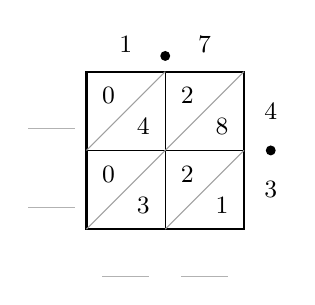
\begin{tikzpicture}[baseline=(current bounding box.north),scale=1.0]
  \lsetup{2}{2}
  \lgrid
  \ltop{1}{1} \ltop{2}{7} \ltopdot{1}
  \lside{1}{4} \lside{2}{3} \lsidedot{1}
  \lcell{1}{1}{0}{4} \lcell{2}{1}{2}{8}
  \lcell{1}{2}{0}{3} \lcell{2}{2}{2}{1}
  \lanslines
\end{tikzpicture}\\[8pt]
$1.7\times4.3=\ansline[2cm]$
\end{minipage}
\end{center}

\item
\begin{ealglossed}
Fill in these \ealgloss{grids}{siatki}, then find where the \ealgloss{decimal point}{przecinek dziesiętny} goes. In part (b)
the \ealgloss{decimal points}{przecinki dziesiętne} are not in the same place in the two numbers, so the two
lines will not meet in the middle of the \ealgloss{grid}{siatka}.
\end{ealglossed}
\vspace{2pt}

\begin{minipage}[t]{0.42\linewidth}
\centering
(a) $0.6\times4.5$\\[4pt]
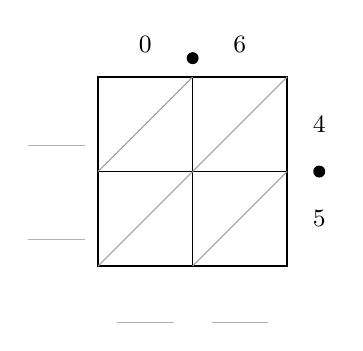
\begin{tikzpicture}[baseline=(current bounding box.north),scale=1.2]
  \lsetup{2}{2}
  \lgrid
  \ltop{1}{0} \ltop{2}{6} \ltopdot{1}
  \lside{1}{4} \lside{2}{5} \lsidedot{1}
  \lanslines
\end{tikzpicture}\\[8pt]
$0.6\times4.5=\ansline[2cm]$
\end{minipage}%
\begin{minipage}[t]{0.58\linewidth}
\centering
(b) $12.4\times0.3$\\[4pt]
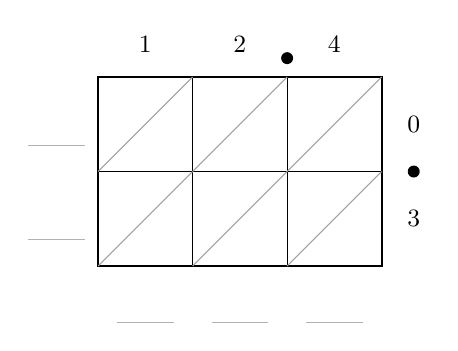
\begin{tikzpicture}[baseline=(current bounding box.north),scale=1.2]
  \lsetup{3}{2}
  \lgrid
  \ltop{1}{1} \ltop{2}{2} \ltop{3}{4} \ltopdot{2}
  \lside{1}{0} \lside{2}{3} \lsidedot{1}
  \lanslines
\end{tikzpicture}\\[8pt]
$12.4\times0.3=\ansline[2cm]$
\end{minipage}

\item
\begin{ealglossed}
Use your answer to Q4 part (a) to write down each of these without
drawing a \ealgloss{grid}{siatka}. Explain how you decided where to put the \ealgloss{decimal point}{przecinek dziesiętny} each
time.
\end{ealglossed}
\begin{multicols}{3}
\begin{enumerate}
  \item $6\times45=\ansline[1.5cm]$
  \item $0.06\times4.5=\ansline[1.5cm]$
  \item $60\times0.45=\ansline[1.5cm]$
\end{enumerate}
\end{multicols}
\vspace{13em}

\end{enumerate}

\newpage

\parttitle{3}{Using the method}

\begin{ealglossed}
The \ealgloss{decimal point}{przecinek dziesiętny} of a \ealgloss{whole number}{liczba całkowita nieujemna} is at the end of its \ealgloss{digits}{cyfry}, so its mark
goes on the corner of the \ealgloss{grid}{siatka}. Everything else about the method stays the
same.
\end{ealglossed}

\begin{enumerate}[resume]

\item
\begin{enumerate}
  \item
        \begin{ealglossed}
        A school orders $24$ packs of pencils. Each pack costs \pounds3.65.
        Use the \ealgloss{grid}{siatka} to work out the total cost of the order.
        \end{ealglossed}
        \vspace{2pt}

        \begin{center}
        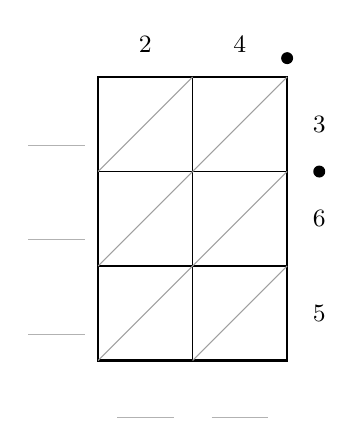
\begin{tikzpicture}[baseline=(current bounding box.north),scale=1.2]
          \lsetup{2}{3}
          \lgrid
          \ltop{1}{2} \ltop{2}{4} \ltopdot{2}
          \lside{1}{3} \lside{2}{6} \lside{3}{5} \lsidedot{1}
          \lanslines
        \end{tikzpicture}
        \end{center}
        \vspace{2pt}
        Total cost: \pounds\ansline[2.5cm]

  \item
        \begin{ealglossed}
        A dripping tap loses $0.35$ litres of water every hour. Use the \ealgloss{grid}{siatka}
        to work out how much water it loses in $16$ hours.
        \end{ealglossed}
        \vspace{2pt}

        \begin{center}
        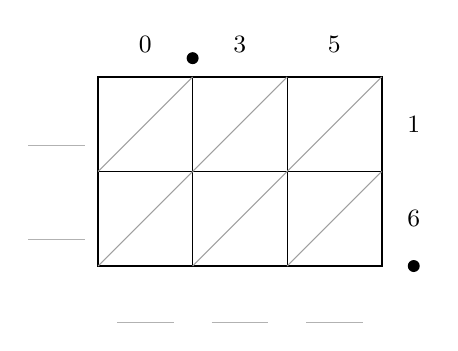
\begin{tikzpicture}[baseline=(current bounding box.north),scale=1.2]
          \lsetup{3}{2}
          \lgrid
          \ltop{1}{0} \ltop{2}{3} \ltop{3}{5} \ltopdot{1}
          \lside{1}{1} \lside{2}{6} \lsidedot{2}
          \lanslines
        \end{tikzpicture}
        \end{center}
        \vspace{2pt}
        Water lost: \ansline[2.5cm] litres
\end{enumerate}

\newpage

\item
\begin{ealglossed}
Draw your own \ealgloss{grid}{siatka} for each of these. Mark the \ealgloss{decimal points}{przecinki dziesiętne} on the
edges of the \ealgloss{grid}{siatka}, and show the \ealgloss{diagonal}{przekątna} you followed to place the \ealgloss{decimal point}{przecinek dziesiętny} in the answer.
\end{ealglossed}
\vspace{2pt}

\begin{minipage}[t]{0.46\linewidth}
(a) Petrol costs \pounds1.45 per litre. Kofi buys $38$ litres. How much does
he pay?

\vspace{13em}
\end{minipage}\hfill
\begin{minipage}[t]{0.46\linewidth}
\begin{ealglossed}
(b) A \ealgloss{rectangular}{prostokątny} tile measures $4.8$ cm by $2.5$ cm. What is its \ealgloss{area}{pole}?
\end{ealglossed}

\vspace{13em}
\end{minipage}

\item
\begin{ealglossed}
\textbf{Practice.} Use the Chinese \ealgloss{multiplication}{mnożyć} method for each of
these, drawing the \ealgloss{grids}{siatki} yourself.
\end{ealglossed}
\begin{multicols}{3}
\begin{enumerate}
  \item $73\times48$
  \item $5.2\times3.6$
  \item $0.9\times0.7$
  \item $126\times34$
  \item $8.4\times0.25$
  \item $1.06\times3.5$
\end{enumerate}
\end{multicols}
\vspace{26em}

\end{enumerate}

\newpage

\parttitle{4}{Challenges}

\begin{enumerate}[resume]

\item
\begin{ealglossed}
\textbf{Why the \ealgloss{diagonals}{przekątne} work.} In the \ealgloss{grid}{siatka} for $47\times36$, the \ealgloss{cell}{komórka}
holding $4\times6$ and the \ealgloss{cell}{komórka} holding $7\times3$ lie on the same \ealgloss{diagonal}{przekątna}.
\end{ealglossed}
\begin{enumerate}
  \item Work out $40\times6$ and $7\times30$. What do you notice about the two
        answers?

        \vspace{6.5em}
  \item
        \begin{ealglossed}
        Use part (a) to explain why the two \ealgloss{cells}{komórki} on that \ealgloss{diagonal}{przekątna} are added
        together.
        \end{ealglossed}

        \vspace{7.5em}
\end{enumerate}

\item
\begin{ealglossed}
Sam uses the method on $0.48\times0.25$. His \ealgloss{digits}{cyfry} come out as
$001200$, and he writes the answer $1200$.
\end{ealglossed}
\begin{enumerate}
  \item
        \begin{ealglossed}
        Without working the \ealgloss{multiplication}{mnożyć} out, explain how you know that
        $1200$ cannot be right.
        \end{ealglossed}

        \vspace{5.5em}
  \item
        \begin{ealglossed}
        Draw the \ealgloss{grid}{siatka}, place the \ealgloss{decimal point}{przecinek dziesiętny}, and write down the correct
        answer.
        \end{ealglossed}

        \vspace{14em}
\end{enumerate}

\newpage

\item
\begin{ealglossed}
How many single-\ealgloss{digit}{cyfra} \ealgloss{multiplications}{mnożyć} does the method need to work out a
three-\ealgloss{digit}{cyfra} number \ealgloss{multiplied}{mnożyć} by a four-\ealgloss{digit}{cyfra} number? Explain how you know
without drawing the \ealgloss{grid}{siatka}.
\end{ealglossed}

\vspace{9em}

\item
\begin{ealglossed}
Design a \ealgloss{multiplication}{mnożyć} of two numbers, each written to one \ealgloss{decimal place}{miejsce dziesiętne}, whose answer is exactly $0.36$. Show that your \ealgloss{multiplication}{mnożyć} works using the Chinese \ealgloss{multiplication}{mnożyć} method.
\end{ealglossed}

\vspace{18em}

\item
\begin{ealglossed}
Zainab says: ``The Chinese \ealgloss{multiplication}{mnożyć} method is better than the
\ealgloss{column method}{metoda kolumnowa}, because you never have to \ealgloss{carry}{przenosić}.''
Use one of your answers from this sheet to decide whether she is right.
\end{ealglossed}

\vspace{13em}

\end{enumerate}

\newpage

\heading{Answers}

{\small
\begin{multicols}{2}
\raggedcolumns
\setlength{\parskip}{4pt}

\begin{ealglossed}
\textbf{Q1.} (a) The \ealgloss{diagonals}{przekątne} give $8$, then $0+0+6=6$, then $2+0+5=7$, then
$1$, so $52\times34=1768$. \quad
(b) The \ealgloss{diagonals}{przekątne} give $6$, then $5+2+2=9$, then $4+3+4=11$, so write $1$ and
\ealgloss{carry}{przenosić} $1$, then $2+1=3$, so $68\times47=3196$.
\end{ealglossed}

\begin{ealglossed}
\textbf{Q2.} (a) The \ealgloss{cells}{komórki} hold $06$, $08$, $15$ and $20$. The \ealgloss{diagonals}{przekątne} give
$0$, then $2+5+8=15$, so write $5$ and \ealgloss{carry}{przenosić} $1$, then $1+0+6+1=8$, then $0$,
so $34\times25=850$. \quad
(b) The \ealgloss{cells}{komórki} hold $02$, $04$ and $03$ along the top \ealgloss{row}{wiersz}, and $14$, $28$ and
$21$ along the bottom \ealgloss{row}{wiersz}. The \ealgloss{diagonals}{przekątne} give $1$, then $2+8+3=13$, then
$2+4+4+0+1=11$, then $1+0+2+1=4$, then $0$, so $243\times17=4131$.
\end{ealglossed}

\begin{ealglossed}
\textbf{Q3.} The \ealgloss{digits}{cyfry} are $0731$. Both \ealgloss{decimal points}{przecinki dziesiętne} sit after the first
\ealgloss{digit}{cyfra} of their number, so the two lines meet in the middle of the \ealgloss{grid}{siatka} and the
\ealgloss{diagonal}{przekątna} leaves the \ealgloss{grid}{siatka} at the bottom left corner: $07.31$, which is $7.31$.
\end{ealglossed}

\begin{ealglossed}
\textbf{Q4.} (a) The \ealgloss{cells}{komórki} hold $00$, $24$, $00$ and $30$. The \ealgloss{digits}{cyfry} are
$0270$ and the \ealgloss{diagonal}{przekątna} leaves the \ealgloss{grid}{siatka} at the bottom left corner, giving
$02.70$, so $0.6\times4.5=2.7$. \quad
(b) The \ealgloss{cells}{komórki} hold $00$, $00$ and $00$ along the top \ealgloss{row}{wiersz}, and $03$, $06$ and
$12$ along the bottom \ealgloss{row}{wiersz}. The \ealgloss{digits}{cyfry} are $00372$. The line down from the top
meets the line in from the side one \ealgloss{column}{kolumna} further to the right, so the
\ealgloss{diagonal}{przekątna} leaves the \ealgloss{grid}{siatka} through the bottom edge, between the third and fourth
\ealgloss{digits}{cyfry}: $003.72$, so $12.4\times0.3=3.72$.
\end{ealglossed}

\begin{ealglossed}
\textbf{Q5.} (a) $270$ \quad (b) $0.27$ \quad (c) $27$. The \ealgloss{digits}{cyfry} of the
answer are $27$ every time, because the \ealgloss{digits}{cyfry} being \ealgloss{multiplied}{mnożyć} have not
changed. Only the \ealgloss{place value}{wartość pozycyjna} changes: in (a) both numbers have been \ealgloss{multiplied}{mnożyć}
by $10$, so the answer is $100$ times larger than $2.7$; in (b) the first
number has been divided by $10$, so the answer is $10$ times smaller; in (c)
the first number has been \ealgloss{multiplied}{mnożyć} by $100$ and the second divided by $10$,
so the answer is $10$ times larger.
\end{ealglossed}

\begin{ealglossed}
\textbf{Q6.} (a) The \ealgloss{digits}{cyfry} are $08760$. The \ealgloss{decimal point}{przecinek dziesiętny} of $24$ is on the
right-hand corner of the \ealgloss{grid}{siatka}, and the \ealgloss{diagonal}{przekątna} from where the two lines meet
leaves the \ealgloss{grid}{siatka} at the bottom left corner, giving $087.60$. The order costs
\pounds$87.60$. \quad
(b) The \ealgloss{digits}{cyfry} are $00560$, and the \ealgloss{decimal point}{przecinek dziesiętny} goes between the third and
fourth of them, giving $005.60$. The tap loses $5.6$ litres.
\end{ealglossed}

\begin{ealglossed}
\textbf{Q7.} (a) $1.45\times38=55.10$, so Kofi pays \pounds$55.10$. \quad
(b) $4.8\times2.5=12.00$, so the \ealgloss{area}{pole} is $12$ cm$^2$. The two zeros after the
\ealgloss{decimal point}{przecinek dziesiętny} do not change the value, so they are not written.
\end{ealglossed}

\textbf{Q8.} (a) $3504$ \quad (b) $18.72$ \quad (c) $0.63$ \quad (d) $4284$
\quad (e) $2.1$ \quad (f) $3.71$

\begin{ealglossed}
\textbf{Q9.} (a) $40\times6=240$ and $7\times30=210$. Both answers are a \ealgloss{whole number}{liczba całkowita nieujemna} of tens, so the \ealgloss{digit}{cyfra} each one contributes lands in the tens \ealgloss{column}{kolumna} of the answer. \quad
(b) A \ealgloss{cell}{komórka} does not really hold $4\times6$; it holds $40\times6$, because the $4$ is in the tens \ealgloss{column}{kolumna}. Every \ealgloss{cell}{komórka} on the same \ealgloss{diagonal}{przekątna} stands for the same \ealgloss{place value}{wartość pozycyjna} in the answer, which is why the \ealgloss{digits}{cyfry} on one \ealgloss{diagonal}{przekątna} are added together, and why a \ealgloss{diagonal}{przekątna} totalling ten or more \ealgloss{carries}{przenosić} into the next \ealgloss{diagonal}{przekątna}.
\end{ealglossed}

\begin{ealglossed}
\textbf{Q10.} (a) $0.48$ is less than $1$ and $0.25$ is less than $1$, so the
answer must be smaller than either of them, and certainly smaller than $1$.
Sam's answer is more than a thousand. \quad
(b) The \ealgloss{digits}{cyfry} are $001200$. The \ealgloss{decimal point}{przecinek dziesiętny} of $0.48$ is after its first
\ealgloss{column}{kolumna} and the \ealgloss{decimal point}{przecinek dziesiętny} of $0.25$ is after its first \ealgloss{row}{wiersz}, so the two lines
meet one \ealgloss{cell}{komórka} in from the top left corner. The \ealgloss{diagonal}{przekątna} from there leaves the \ealgloss{grid}{siatka} through the left-hand side, between the second and third \ealgloss{digits}{cyfry}, giving
$00.1200$. So $0.48\times0.25=0.12$.
\end{ealglossed}

\begin{ealglossed}
\textbf{Q11.} $12$ \ealgloss{multiplications}{mnożyć}. The \ealgloss{grid}{siatka} has one \ealgloss{column}{kolumna} for each of the three \ealgloss{digits}{cyfry} and one \ealgloss{row}{wiersz} for each of the four \ealgloss{digits}{cyfry}, so it has $3\times4=12$ \ealgloss{cells}{komórki}, and each \ealgloss{cell}{komórka} holds one single-\ealgloss{digit}{cyfra} \ealgloss{multiplication}{mnożyć}.
\end{ealglossed}

\begin{ealglossed}
\textbf{Q12.} Many answers. For example $0.4\times0.9$, $0.6\times0.6$,
$1.2\times0.3$ and $1.8\times0.2$ all give $0.36$. The \ealgloss{digits}{cyfry} of the two
numbers have to \ealgloss{multiply}{mnożyć} to $36$, and each number has one \ealgloss{digit}{cyfra} after the
\ealgloss{decimal point}{przecinek dziesiętny}, so the answer has two.
\end{ealglossed}

\begin{ealglossed}
\textbf{Q13.} She is partly right. No \ealgloss{carrying}{przenosić} happens while the \ealgloss{grid}{siatka} is being
filled in, because every \ealgloss{cell}{komórka} holds a single-\ealgloss{digit}{cyfra} \ealgloss{multiplication}{mnożyć} and its two
\ealgloss{digits}{cyfry} have a triangle each. \ealgloss{Carrying}{przenosić} does still happen when the \ealgloss{diagonals}{przekątne}
are added: in Q1 part (b) the third \ealgloss{diagonal}{przekątna} came to $11$, so the $1$ had to be
\ealgloss{carried}{przenosić} into the next \ealgloss{diagonal}{przekątna}.
\end{ealglossed}

\end{multicols}
}

\end{document}